\chapter{Implementation}

\section{Architecture (MVVM)}
\section{IPC?}
\section{Permissions \& Android Manifest}

\section{Implementation of Concerns}

\subsection{Recording}
\subsection{Sharing}

\subsection{Modules}
Modules have three actions: A) retrieve/display modules; B) install modules; and C) launch module. 

In Figure \ref{fig:impl_modules}, the method calls and the interactions between the components are shown.  Based on the actions: 

\begin{itemize}
    \item[A.1] Test
    \item[A.2] Test
    \item[A.3] Test
    \item[A.4] Test
    \item[B.1] Test
    \item[B.2] Test
    \item[B.3] Test
    \item[B.4] Test
    \item[B.5] Test
    \item[B.6] Test
    \item[C.1] Test 
    \item[C.2]     
\end{itemize}

\begin{figure}
    \centering
    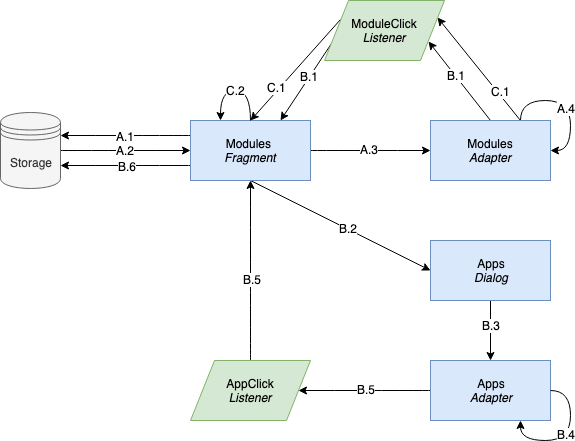
\includegraphics[scale=0.6]{images/Module_Imp.png}
    \caption{Implementation of module functionality}
    \label{fig:impl_modules}
\end{figure}

\subsubsection{Data Exchange Implementation}
\begin{lstlisting}[language=json, caption={My Caption}, captionpos=b]
public void onLaunchModuleClick(String packageName) {
    Intent moduleApplication = context.getPackageManager().getLaunchIntentForPackage(packageName);
    
    if (moduleApplication == null) return;

    String data = formatAllRecordsToJSON();

    Bundle bundle = new Bundle();
    bundle.putString("data", data);

    moduleApplication.putExtras(bundle);

    startActivity(moduleApplication);
}

\end{lstlisting}



\subsection{Analytics}
\begin{figure}
    \centering
    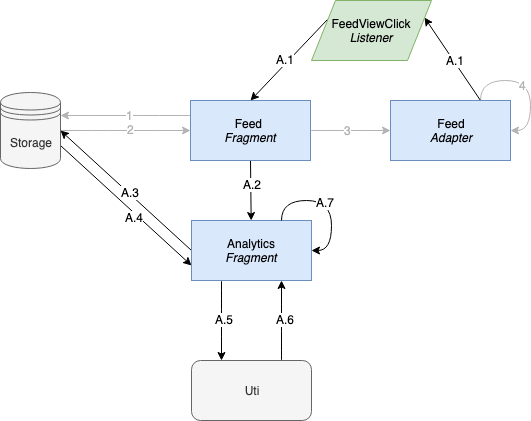
\includegraphics[scale=0.6]{images/Anal_Imp.png}
    \caption{Implementation of analytics functionality}
    \label{fig:impl_analytics}
\end{figure}


\subsection{Storage}
\subsection{Presentation}

